% Figure: 17x17 confusion matrix, ConvNeXt-Tiny, counts summed over 3 seeds
% Source     : docs/reports/experiments/phase_1b/final_b_new_recomputed/
%              20260819T043733Z/predictions.csv   (only source of the counts)
% Cross-check: confusion_matrices.npz, exact element-wise after permuting to
%              the family class order -- 0 cells differing on all three seeds
% Artifacts  : artifact/person3/confusion/{confusion_convnext_main.csv,
%              confusion_convnext_main_per_seed.csv, confusion_metadata.json}
% Run ids    : taskB17__main__seed_{42,123,456}__convnext_tiny
\begin{figure}[!htbp]
\centering
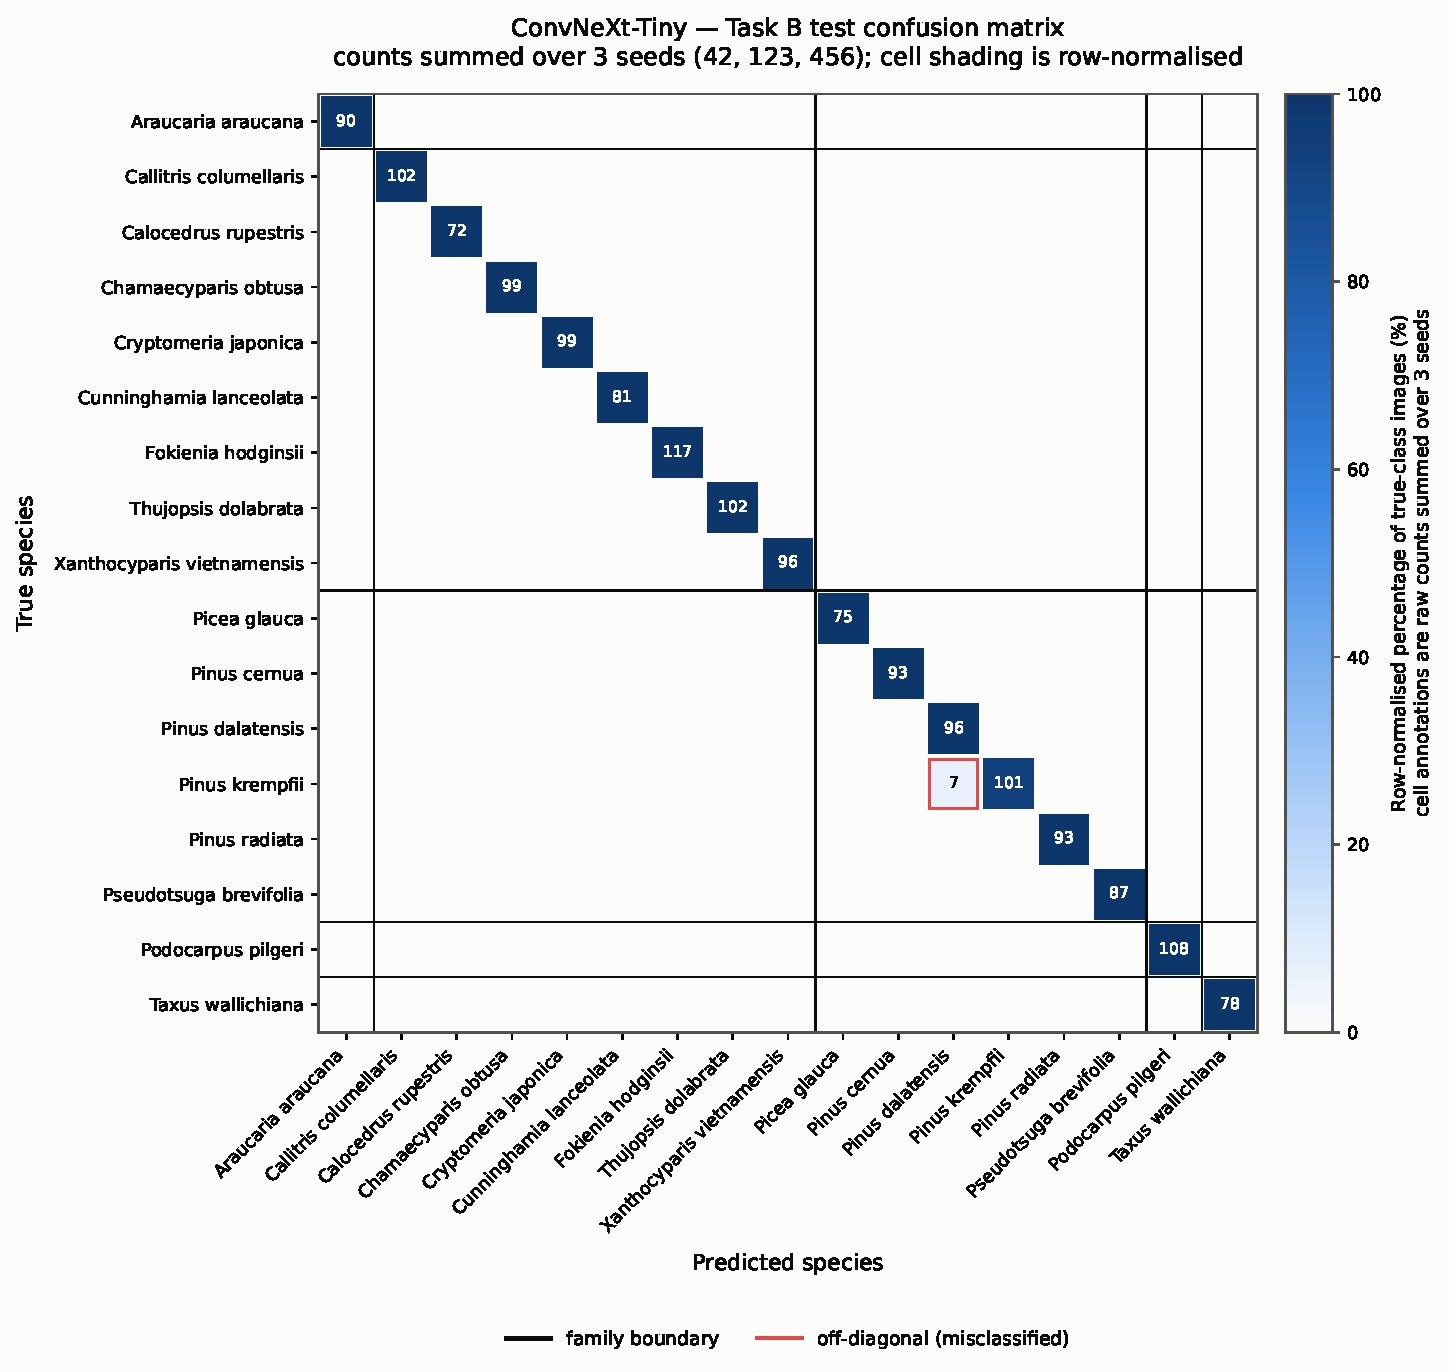
\includegraphics[width=\columnwidth]{artifact/person3/confusion/fig_confusion.pdf}
\caption{Ma trận nhầm lẫn của ConvNeXt-Tiny trên tập test Task~B. Các count được cộng theo từng phần tử qua ba seed chính (42, 123, 456), cho $532\times3 = 1{,}596$ dự đoán; mỗi seed đóng góp như nhau. Màu nền ô là tỷ lệ phần trăm đã chuẩn hóa theo hàng của số ảnh thuộc lớp thật, với mẫu số là tổng hàng của các count đã cộng; số ghi trong mỗi ô là count thô đã cộng. Các loài được sắp theo họ và các đường kẻ đen đánh dấu ranh giới họ. Ô ngoài đường chéo được viền đỏ. ConvNeXt-Tiny được chọn theo tiêu chí cố định trước (macro-F1 trung bình cao nhất trên ba seed ở Bảng~\ref{tab:task_b}), chứ không phải bằng cách xem ma trận này. Ba ma trận riêng từng seed được công bố kèm bản gộp để kiểm tra lại được phép cộng.}
\label{fig:confusion}
\end{figure}
